% begin module EVT-statement
\begin{frame}[t]
\begin{theorem}[The Extreme Value Theorem]
If  $f$ is continuous on a closed and bounded interval $[a,b]$, then $f$ attains its maximum and minimum value, each at least once. In other words, there exist numbers $c$ and $d$ in $[a,b]$ such that 
\[
f(c)\geq f(x)\geq f(d) \quad \quad \quad \text{for~all~}x\in[a,b]
\]
\end{theorem}
\begin{columns}[c]
\column{.3\textwidth}
\ \uncover<2->{%
\psset{xunit=0.6cm, yunit=0.6cm}
\begin{pspicture}(-0.5,-0.8)(5.4,3.4)
\psframe*[linecolor=white](-0.5,-0.8)(5.4,3.4)
\psaxes[ticks=none, labels=none]{<->}(0,0)(-0.5,-0.8)(5.2,3.2)\tiny
\psLabels{5.2}{3.2}
%Function formula: (-3/4+1/2 (x))^{2}+1 
\psplot[linecolor=red, plotpoints=1000]{0.5}{4}{1 x 0.5 mul -0.75 add 2 exp add }
\psFullDot{0.5}{1.25}
\psFullDot{4}{2.5625}
\psline[linestyle=dashed](1.5,0)(1.5,1)
\psline[linestyle=dashed](4,0)(4,2.5625)
\psXTick{0.5}
\rput[t](0.5, -0.2){$a$}
\psXTick{1.5}
\rput[t](1.5, -0.2){$d$}
\psXTick{4}
\rput[t](4, -0.2){$c=b$}
\end{pspicture} 
%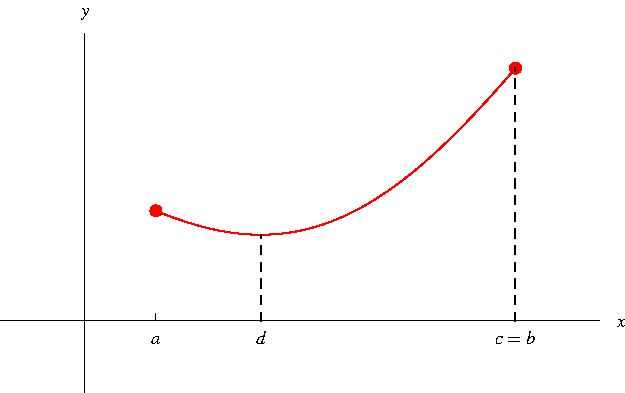
\includegraphics[width=4cm]{maxima-minima/pictures/04-01-evtb.pdf}%
}%
\column{.3\textwidth}
\psset{xunit=0.6cm, yunit=0.6cm}
\begin{pspicture}(-0.5,-0.8)(5.3,3.3)
\psframe*[linecolor=white](-0.5,-0.8)(5.3,3.3)
\psaxes[ticks=none, labels=none]{<->}(0,0)(-0.5,-0.8)(5.2,3.2)\tiny
\psLabels{5.2}{3.2}
%Function formula: 1/2+3 (x)+1/6 ((x)^{3})-11/8 ((x)^{2}) 
\psplot[linecolor=red, plotpoints=1000]{0.5}{4.8}{x 2 exp -1.375 mul x 3 exp 0.166667 mul x 3 mul 0.5 add add add }
\psFullDot{0.5}{1.67708}
\psFullDot{4.8}{1.652}
\psline[linestyle=dashed](1.5,0)(1.5,2.46875)
\psline[linestyle=dashed](4,0)(4,1.16667)
\psXTick{0.5}
\rput[t](0.5, -0.2){$a$}
\psXTick{1.5}
\rput[t](1.5, -0.2){$c$}
\psXTick{4}
\rput[t](4, -0.2){$d$}
\psXTick{4.8}
\rput[t](4.8, -0.2){$b$}
\end{pspicture} 
%\ 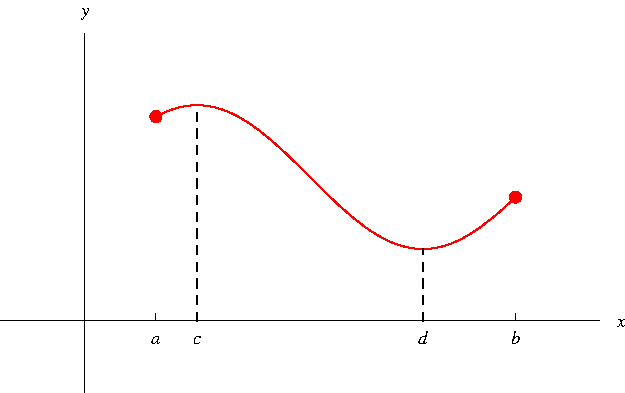
\includegraphics[width=4cm]{maxima-minima/pictures/04-01-evta.pdf}%
\column{.3\textwidth}
\ \uncover<3->{%
\psset{xunit=0.6cm, yunit=0.6cm}
\begin{pspicture}(-0.5,-0.8)(5.3,3.3)
\psframe*[linecolor=white](-0.5,-0.8)(5.3,3.3)
\psaxes[ticks=none, labels=none]{<->}(0,0)(-0.5,-0.8)(5.2,3.2)\tiny
\psLabels{5.2}{3.2}
%Function formula: -3/2+10 (x)+5/2 ((x)^{3})-1/4 ((x)^{4})-33/4 ((x)^{2}) 
\psplot[linecolor=red, plotpoints=1000]{0.5}{4.5}{x 2 exp -8.25 mul x 4 exp -0.25 mul x 3 exp 2.5 mul x 10 mul -1.5 add add add add }
\psline[linestyle=dashed](1,0)(1,2.5)
\psline[linestyle=dashed](2.5,0)(2.5,1.23438)
\psline[linestyle=dashed](4,0)(4,2.5)

\psFullDot{0.5}{1.73438}
\psXTick{0.5}
\rput[t](0.5, -0.2){$a$}

\psXTick{1}
\rput[t](1, -0.2){$c_1$}

\psXTick{4}
\rput[t](4, -0.2){$c_2$}

\psXTick{2.5}
\rput[t](2.5, -0.2){$d$}

\psXTick{4.5}
\psFullDot{4.5}{1.73438}
\rput[t](4.5, -0.2){$b$}
\end{pspicture} 
%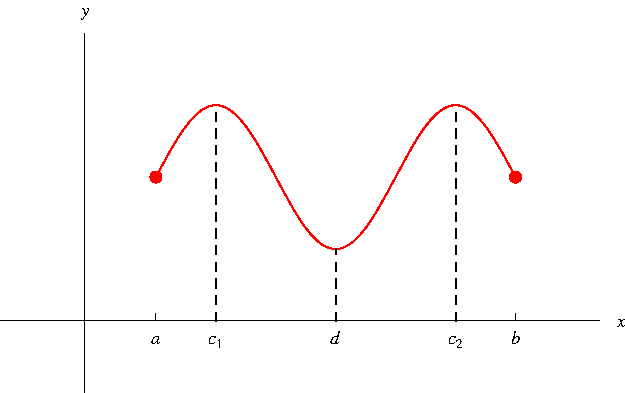
\includegraphics[width=4cm]{maxima-minima/pictures/04-01-evtc.pdf}%
}%
\end{columns}
\begin{itemize}
\item<2-| alert@2>  Extreme values might happen at endpoints.
\item<3-| alert@3>  Extreme values might happen twice.
\end{itemize}
\end{frame}
% end module EVT-statement
